\section{Classical evaluators, Turing's method and the P\'olya route}\label{ch:classical}

The classical evaluators on the critical line pay for height differently and, at large height, far less than the P\'olya route, tilted or not.

\subsection{The Riemann Siegel formula, Gram points and certified counts}\label{sec:ch5:turing}

On the critical line $\zeta(\frac12+it)=e^{-i\vartheta(t)}Z(t)$, where $\vartheta(t)=\im\log\Gamma(\frac14+\frac{it}2)-\frac t2\log\pi$ is the Riemann Siegel theta function and $Z(t)$ is real for real $t$. Write $m=\lfloor\sqrt{t/2\pi}\rfloor$ and $q=\sqrt{t/2\pi}-m$. For every $K\ge0$,
\[
Z(t)=2\sum_{n\le m}\frac{\cos(\vartheta(t)-t\log n)}{\sqrt n}+(-1)^{m-1}\Big(\frac t{2\pi}\Big)^{-1/4}\sum_{j=0}^{K}C_j(q)\Big(\frac t{2\pi}\Big)^{-j/2}+R_K(t),
\]
where $R_K(t)=O(t^{-(2K+3)/4})$ as $t\to\infty$, $C_0(q)=\cos(2\pi(q^2-q-\frac1{16}))/\cos(2\pi q)$, and the higher $C_j$ are given in \cite[Section 7.5]{Edwards} and \cite{Gabcke79}. This asymptotic expansion was found in Riemann's unpublished notes and published by Siegel \cite{Siegel32}.

The main sum is the approximate functional equation $\zeta(s)=\sum_{n\le x}n^{-s}+\chi(s)\sum_{n\le y}n^{s-1}+\cdots$, where $\zeta(s)=\chi(s)\zeta(1-s)$ and $2\pi xy=t$ \cite[Chapter 4]{Titchmarsh}, taken at $x=y=\sqrt{t/2\pi}$ and written for $Z$; the $C_j$ correct for the abrupt truncation at $n=m$. The terms are bounded by $2$ and there is no exponential cancellation, so double precision suffices at every height computed in this book; near height $10^{12}$ and above, the phases $\vartheta(t)-t\log n$ must be reduced modulo $2\pi$ in higher precision. Gabcke's thesis gives explicit bounds for the remainders $R_K$ with $K\le10$ \cite{Gabcke79}, and with them the formula can be used in rigorous computation.

To evaluate $Z$ at many points near height $T$, Odlyzko and Sch\"onhage \cite{OS88} compute the main sum on a grid by fast Fourier transforms and rational function evaluation, and interpolate between grid points by band limited interpolation. About $T^{1/2}$ values then cost $T^{1/2+o(1)}$ operations, that is $T^{o(1)}$ per point. Odlyzko compared the spacings of the zeros near zero number $10^{12}$ with the Gaussian unitary ensemble \cite{Odlyzko87}, and with the algorithm he later took such computations to zero numbers $10^{20}$ \cite{Odlyzko92} and $10^{22}$ \cite{Odlyzko01}.

The classical searches for zeros on the line sample $Z$ at the Gram points $g_n$, defined by $\vartheta(g_n)=n\pi$ \cite[pp.~301 and 302]{Gram03}. There $Z(g_n)$ usually has the sign of $(-1)^n$, and each Gram interval $[g_{n-1},g_n)$ usually contains exactly one zero. This is Gram's law, and it fails with positive frequency \cite[Corollary 5.4]{Trudgian11b}. Call $g_n$ good when $(-1)^nZ(g_n)>0$, and call an interval $[g_j,g_{j+k})$ between consecutive good Gram points a Gram block. Rosser's rule asserts that such a block contains exactly $k$ zeros \cite{RYS69}, \cite[Section 7.3]{Trudgian11b}. It holds far longer than Gram's law, since its first exception is the block that begins at $g_{13\,999\,525}$ \cite[Table 3]{Brent79}, but it too fails with positive frequency \cite[Corollary 7.8]{Trudgian11b}. Counting sign changes of $Z$ gives a lower bound for the number of zeros on the line. The difficulty is to show that none is missing, whether off the line or in a close pair that produces no sign change.

Turing's answer \cite{Turing53} uses the counting function $N(T)=\vartheta(T)/\pi+1+S(T)$, where, for $T$ not an ordinate, $\pi S(T)=\arg\zeta(\frac12+iT)$, the argument being defined by continuous variation along $2\to2+iT\to\frac12+iT$. The function $S$ is small on average: Littlewood proved $\int_0^TS(t)\,dt=O(\log T)$ \cite[Theorem 9.9(A)]{Titchmarsh}, and Turing gave explicit constants for $|\int_{t_1}^{t_2}S(t)\,dt|$, later sharpened by Trudgian \cite{Trudgian11}. If the sign changes found near height $T$ were fewer than $N(T)$, then $S$ would be displaced by at least $2$ over an interval long enough to violate the integral bound. The count is therefore certified by locating the sign changes in a range slightly beyond $T$ and checking them against Turing's bound for $\int S$. The method never evaluates $\zeta$ off the line. Turing's published argument contained errors, corrected by Lehman \cite{Lehman70}, and the corrected method underlies every large verification since, including Platt and Trudgian's to height $3\times10^{12}$ \cite{PT21}.

Before Turing, counts were certified by Backlund's method. Since $\re\zeta(2+it)\ge2-\zeta(2)>0$ for every $t$, it suffices to check that $\re\zeta(\sigma+iT)\ne0$ for $\frac12\le\sigma\le2$: then $\arg\zeta$ stays in $(-\frac\pi2,\frac\pi2)$ along the whole path, so $|S(T)|<\frac12$ and $N(T)$ is the integer nearest to $\vartheta(T)/\pi+1$. Backlund carried this out for $T=200$ \cite{Backlund} and Hutchinson for $T=300$ \cite[pp.~54 to 57]{Hutchinson25}, \cite{Trudgian11}.

\subsection{The P\'olya route beside the classical evaluators}

The P\'olya route evaluates $\xi$ and $\xi'$ on and off the line, at $\tfrac12+\varepsilon+i\theta$, from the P\'olya kernel, and so delivers the Thorin density $\rho_\varepsilon$, its mass and the zero count from one evaluator. Its count has the logic of Turing's certificate: when the sign changes of $\Xi$ and the argument principle count $N(T)$ agree, every zero up to height $T$ is on the line and simple (Section~\ref{sec:ch4:height200}).

The methods differ most in how their cost grows with height (Table~\ref{tab:compare}). The untilted P\'olya route needs about $0.341\,t$ extra digits; and by the budget of Section~\ref{sec:ch4:trapezoid} its step must be below $\pi/t$, so that its number of nodes grows linearly with $t$ as well. The cause is aliasing. By Poisson summation the trapezoid sum at $s=\varepsilon+it$ equals $\sum_{k\in\mathbb Z}\xi(\frac12+s-2\pi ik/h)$, and the term $k=1$, at height $t-2\pi/h$, is exponentially larger than $\xi(\frac12+s)$ once $t>\pi/h$. The tilted contour of Section~\ref{sec:newcomp} cuts the loss of digits to about $\delta t/\log10$, but aliasing still requires $2\pi/h>t$, by the second condition in \eqref{eq:ch4:tiltcond}, so there too the number of nodes grows linearly with $t$.

\begin{table}[t]
\centering\footnotesize
\begin{tabular}{p{0.144\linewidth}p{0.2\linewidth}p{0.2\linewidth}p{0.325\linewidth}}
\toprule
 & \raggedright Riemann Siegel and Turing & Odlyzko Sch\"onhage & P\'olya route\tabularnewline
\midrule
object & sign changes of $Z(t)$ & zeros in blocks, statistics & Thorin density $\rho_\varepsilon$, mass, count\\
where evaluated & critical line & critical line & line $\re s=\tfrac12+\varepsilon$ and contour\\
count certificate & Gram points and $\int S$ & Turing's method & argument principle count equal to the number of sign changes; computed, not yet certified\\
cost per point & $\sqrt{t/2\pi}$ terms, double & amortised, $t^{o(1)}$ & $0.341\,t$ extra digits and step below $\pi/t$ (untilted); $\delta t/\log10$ digits and step below $2\pi/t$ (tilted)\\
accuracy & asymptotic remainder & asymptotic remainder & spectral; rounding certified by balls\\
reach & $t\approx1540$ in 1953 & $t\approx10^{20}$ and beyond \cite{Odlyzko92,Odlyzko01} & $t\approx7005$ (Section~\ref{sec:ch5:lehmer}); $25$ digits at $t=5000$ (Table~\ref{tab:tilt})\\
\bottomrule
\end{tabular}
\caption{The Riemann Siegel formula with Turing's method, the Odlyzko Sch\"onhage algorithm and the P\'olya route: what each computes, where, with what certificate, at what cost per point, and how far it has reached.}
\label{tab:compare}
\end{table}

\label{sec:ch5:hybrid}The distances of Section~\ref{ch:distances} do not depend on how $\xi$ is evaluated, and this suggests a hybrid at large height. The approximate functional equation holds off the critical line \cite[Chapter 4]{Titchmarsh}, so Riemann Siegel type expansions of $\zeta$ \cite[Theorems 3.1 and 4.2]{AriasDeReyna11} and of $\zeta'$, and the Odlyzko Sch\"onhage algorithm for blocks of points, apply at $\tfrac12+\varepsilon+i\theta$ as well. With them as the evaluator and Odlyzko's zeros \cite{OdlyzkoTables} as the RH reference, one could compute $\rho_\varepsilon$, the matched total variation and the positivity margin at the heights of Odlyzko's computations, from about $10^{11}$ to beyond $10^{20}$, while the tilted P\'olya route supplies values with explicitly bounded errors on low windows.

\subsection{Two computations beyond the untilted route}

\subsubsection{A Lehmer pair near height 7005}\label{sec:ch5:lehmer}

Lehmer found two zeros that are unusually close, $\gamma_{6709}=7005.0629$ and $\gamma_{6710}=7005.1006$ \cite[pp.~297 and 298]{Lehmer56}, at distance $0.0377$, the classical example of a Lehmer pair; such pairs give lower bounds for the de Bruijn Newman constant \cite{CSV94} (Section~\ref{sec:ch21:bounds}). The untilted P\'olya route cannot reach this height: it would need about $2400$ digits and a step below $4.5\times10^{-4}$. The tilted route with $\delta=0.01$, $256$ bits, $13001$ nodes, step $6\times10^{-4}$ and truncation $|x|\le3.9$ computes $\Xi(\theta)e^{\pi\theta/4}$ at $34$ milliseconds per point. On a grid of step $0.005$ it finds sign changes in $(7005.060,7005.065)$ and $(7005.100,7005.105)$, the two members of the pair (Figure~\ref{fig:ch5:lehmer}).

The Thorin density shows what resolution separates them. A single zero on the line produces a Cauchy peak of height $1/(\pi\varepsilon)$, that is $6.4$, $15.9$ and $31.8$ at $\varepsilon=0.05$, $0.02$ and $0.01$. The largest values of $\rho_\varepsilon$ on the grid are $11.18$, $19.58$ and $33.89$. At $\varepsilon=0.05$ the two peaks have merged into one of nearly double height; at $\varepsilon=0.02$ they are partly separated; at $\varepsilon=0.01$ each carries its own peak, lifted slightly by its neighbour. The Cauchy kernel predicts this: two kernels with half width at half maximum $\varepsilon$ at distance $g$ have a single maximum when $g\le2\varepsilon/\sqrt3$ and two maxima when $g>2\varepsilon/\sqrt3$. With $g=0.0377$ the pair is resolved as two peaks for $\varepsilon<\sqrt3\,g/2\approx0.033$. The criterion concerns two isolated kernels; Exercise~\ref{ex:ch5:cauchy} proves it and asks how much the other zeros move the threshold.

\begin{figure}[htbp]
\centering
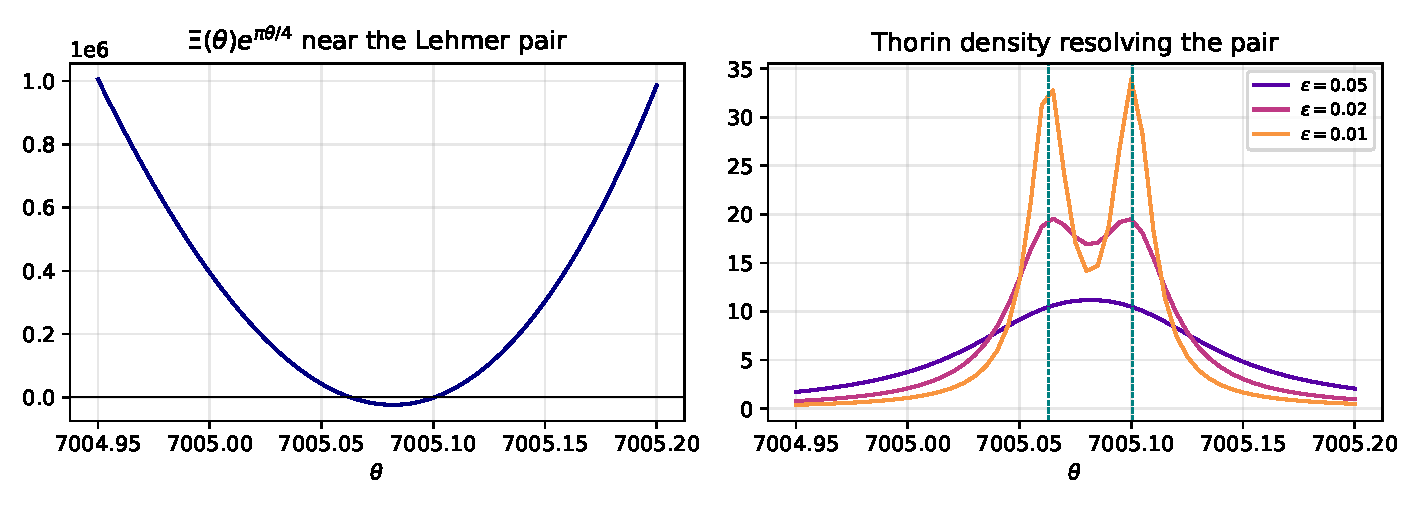
\includegraphics[width=\textwidth]{fig/lehmer.pdf}
\caption{The Lehmer pair near $7005$ computed by the tilted P\'olya route: $\Xi(\theta)e^{\pi\theta/4}$ (left) and the Thorin density at three resolutions (right), drawn through values on a grid of step $0.005$, with the two ordinates dashed.}
\label{fig:ch5:lehmer}
\end{figure}

\subsubsection{The zero count at height 1000}\label{sec:ch5:count}

Proposition~\ref{prop:zerodensity} of Section~\ref{ch:turing} gives the unconditional count $N(T)=M_{1/2}(T)+\tau_{1/2}(T)$, where $M_{1/2}(T)=\pi^{-1}\arg\xi(1+iT)$ is the cumulative Thorin mass at resolution $\frac12$, that is at the basepoint one of Section~\ref{ch:basepoint}, and $\tau_{1/2}(T)$ is $\pi^{-1}$ times the change of $\arg\xi$ along the segment from $1+iT$ to $\frac12+iT$. With the tilted route ($\delta=0.1$, $200$ bits, step $0.004$ and truncation $|x|\le4.2$, that is $2101$ nodes), $10000$ steps of $0.1$ along $\re s=1$ and $2000$ steps along the segment, we find
\[
M_{1/2}(1000)=648.7562315041018,\qquad \tau_{1/2}(1000)=0.2437684958980,
\]
\[
M_{1/2}(1000)+\tau_{1/2}(1000)=648.9999999999999,
\]
so $N(1000)=649$, with a largest argument increment of $0.43$ radians. The computation took $77.5$ seconds; \texttt{mpmath}'s \texttt{nzeros} returns $649$ in $0.017$ seconds. Where Backlund bounds the argument, this computation accumulates it from samples, and ball arithmetic certifies the rounding in each sampled value but not the absence of winding between samples. The count is therefore computed rather than certified. Certifying it would need, besides the analytic error bounds of Section~\ref{ch:polya}, an enclosure of $\xi$ between consecutive sample points $s_k$ and $s_{k+1}$, for instance a check that $\re\,\xi(s)/\xi(s_k)>0$ on a ball containing the segment between them.

For counting and locating zeros at height, the Riemann Siegel family with Turing's method is faster by orders of magnitude, and the P\'olya route is not a competitor there. It reads the count as an integer from a smooth quantity, the Thorin mass, with no Gram point bookkeeping; it gives the zero density strip by strip (Section~\ref{ch:turing}); and it evaluates objects that the classical methods, used on the critical line, do not compute: Thorin densities and their distances to $U_{\RH}$.
